\documentclass[landscape,twocolumn]{article}
\usepackage{german}
\usepackage[latin1]{inputenc}
\usepackage{dcolumn}
\usepackage{longtable}
\usepackage{amsmath}
\usepackage{amssymb}
\usepackage{wrapfig}
\usepackage{epsfig}
\usepackage{fancyheadings}
\usepackage{multirow}
\usepackage{tabularx}

\textheight=16.2cm \textwidth=25 cm \evensidemargin=\oddsidemargin
\setlength{\headsep}{25pt}


\font \tams  = cmmib10   scaled \magstep1 \font \tamss =cmmib10
\font \tenbfne = cmb10   scaled \magstep1 \font \sevenbfne = cmb10
\def\vek#1{\ifmmode{\textfont1=\tams\scriptfont1=\tamss
              \textfont0=\tenbfne\scriptfont0=\sevenbfne
              \mathchoice{\hbox{$\displaystyle#1$}}{\hbox{$\textstyle#1$}}
              {\hbox{$\scriptstyle#1$}}{\hbox{$\scriptscriptstyle#1$}}}
            \else \vrule width 4pt\ #1\ \fi}



 \setlength{\parindent}{0pt}
 \setlength{\voffset}{-0.8in}
 \setlength{\hoffset}{-0.088in}
 \setlength{\columnsep}{1cm}



\begin{document}
\setlength{\extrarowheight}{4pt} \pagestyle{fancyplain}
 \lhead[]{\large  Physikalisches
Anf\"{a}ngerpraktikum der Universit\"{a}t Heidelberg - Praktikum II}
\rhead{\large Versuch 223 Brownsche Bewegung}

\cfoot{\large\vspace{0.1in}$\qquad$\rm\thepage}
\lfoot{\copyright~Dr. J.Wagner - Physikalisches Anf\"{a}ngerpraktikum
-~V.~1.2~B.Sc.~Stand~01/2015} \setlength{\footrulewidth}{0.4pt}
\renewcommand{\thesection}{\Roman{section}}


\begin{center}
\LARGE\bf{Versuch 223\\ Messung der Boltzmannkonstante\\ Teil I
Brownsche Bewegung}
\end{center}

\begin{figure}[h]
\begin{minipage}[c]{12cm}
\centering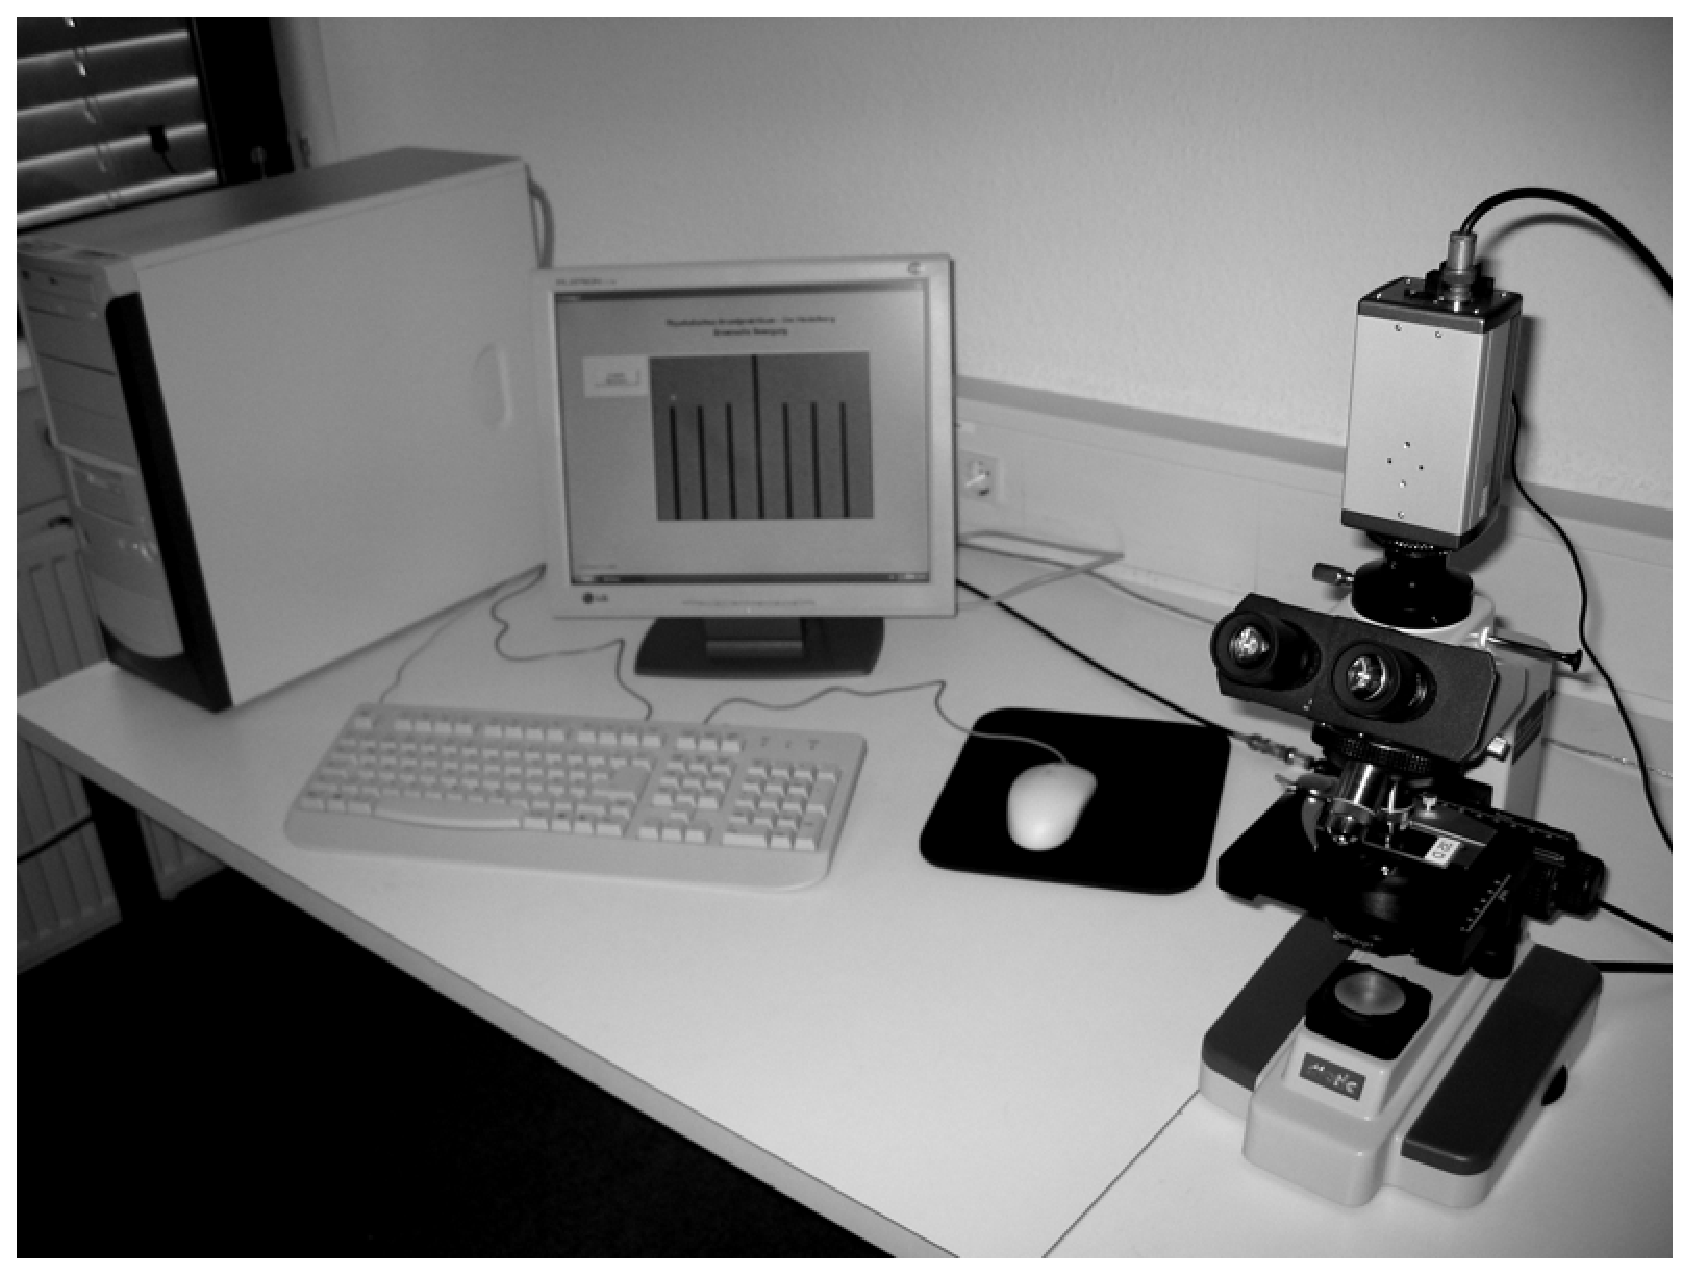
\epsfig{file=249_aufbau.eps,width=\textwidth}
\caption{\fontsize{10}{12}\it Versuchsaufbau.}
\end{minipage}
\end{figure}


\section{Messaufbau}
\begin{itemize}
 \item Durchlichtmikroskop Motic~B1 mit CCD-Kamera
 \item Kugelf\"{o}rmige Partikel suspendiert in Wasser
 \item PC mit Drucker
 \item Thermometer
 \item Objektmikrometer
\end{itemize}


\section{Literatur}

\begin{itemize}
\item Standardwerke der Physik: Gerthsen, Demtr\"{o}der,
Bergmann-Sch\"{a}fer, Tipler.
 \item Die Grundlagen  zu den wichtigsten Wahrscheinlichkeitsverteilungen k\"{o}nnen Sie in der Versuchsbeschreibung des Versuchs~251: \it
 Statistik des radioaktiven Zerfalls\rm~nachlesen.
 \item  Homepage des Praktikums\\
http://www.physi.uni-heidelberg.de/Einrichtungen/AP/
\end{itemize}





\section{Vorbereitung}
Bereiten Sie sich  auf die Beantwortung von Fragen zu folgenden
Themen vor: Kinetische Theorie der W\"{a}rme, Brownsche Bewegung,
Grundlagen der Wahrscheinlichkeitsrechnung und Statistik,
Binomial- und Gau{\ss}-Verteilung.
\\Verst\"{a}ndnisfragen:
\begin{enumerate}
\item Was ist W\"{a}rme aus Sicht der kinetischen Theorie der W\"{a}rme?
Was besagt der Gleichverteilungssatz? Wie hoch ist die thermische
Geschwindigkeit eines Partikels der Masse 10$^{-15}$~kg bei
Zimmertemperatur?

\item Berechnen Sie das Produkt $kT$ f\"{u}r Zimmertemperatur und
geben Sie diesen in der Einheit $eV$ an. Diesen Wert sollten Sie
sich f\"{u}r die Zukunft unbedingt merken.

\item Was bezeichnet man als Brownsche Bewegung? Worin liegt die
Ursache dieser Bewegung? Welche Gr\"{o}{\ss}en haben Einfluss auf die
Brownsche Bewegung?

\item Wie gro{\ss} ist der zu erwartende Wert der mittleren
Verschiebung bzw. der mittleren quadratischen Verschiebung eines
Partikels.

\item Berechnen Sie die mittlere quadratische Verschiebung eines
Partikels (Partikelradius a=500~nm) suspensiert in Wasser
(T=20$^\circ$C) innerhalb eines Zeitraums von t=1~s. Die
Viskosit\"{a}t von Wasser k\"{o}nnen Sie Abbildung~\ref{249_Viskositaet}
entnehmen.

\end{enumerate}

\section{Aufgaben}
\begin{enumerate}
\item Pr\"{a}parieren Sie eine Mikroskopprobe einer Partikelsuspension. 
\item Nehmen Sie jede
Sekunde und mindestens 150 Mal das Mikroskopbild eines einzelnen
Partikels auf. \item Bestimmen Sie den Abbildungsma{\ss}stab des
Mikroskops mit einem Objektmikrometer.
 \item Vermessen Sie die Position des
Partikels anhand der aufgenommenen Bilder. \item Berechnen Sie aus
der mittleren quadratischen Verschiebung die Diffusionskonstante
und die Boltzmannkonstante.
\end{enumerate}

\section{Motivation}
\bf  Mit Bl\"{u}tenpollen l\"{a}{\ss}t sich die Existenz von Atomen und
Molek\"{u}len beweisen \it\\
\\\glqq Heute vor 100 Jahren, am 11. Mai 1905, reichte Albert
Einstein bei den ''Annalen der Physik'' eine wichtige Arbeit ein,
in der er die sogenannte Brownsche Bewegung erkl\"{a}rte. Dem
schottischen Botaniker Robert Brown war bereits im Jahr 1827
aufgefallen, da{\ss} Bl\"{u}tenpollen in einem Glas Wasser eine
eigenartige Zickzackbewegung ausf\"{u}hren. Was war die Ursache daf\"{u}r?
Alle Versuche, diese Brownsche Bewegung zu erkl\"{a}ren, scheiterten
zun\"{a}chst. Sie blieb jahrzehntelang geheimnisvoll. Erst Albert
Einstein erkannte, da{\ss} die Bewegung der kleinen Teilchen in der
Fl\"{u}ssigkeit durch ein fortw\"{a}hrendes Sto{\ss}en der Wassermolek\"{u}le
verursacht wird. Dies war in jener Zeit tats\"{a}chlich noch ein
gewichtiges Argument f\"{u}r die Existenz von Atomen und Molek\"{u}len,
die im 19. Jahrhundert noch heftig umstritten gewesen ist. Und
gleichzeitig pa{\ss}te Einsteins Beschreibung zur molekularen Theorie
der W\"{a}rme. Je w\"{a}rmer beispielsweise Wasser ist, um so gr\"{o}{\ss}er ist
die mittlere Geschwindigkeit, mit der die Wassermolek\"{u}le
ungeordnet umherflitzen und damit St\"{o}{\ss}e verursachen k\"{o}nnen. So
erkl\"{a}rt sich auch der Begriff Thermodynamik: W\"{a}rme ist eben etwas
Dynamisches. Einstein schrieb damals an einen Freund, da{\ss} ''unter
der Voraussetzung der molekularen Theorie der W\"{a}rme in
Fl\"{u}ssigkeiten suspendierte K\"{o}rper von der Gr\"{o}{\ss}enordnung 1/1000
Millimeter bereits eine wahrnehmbare ungeordnete Bewegung
ausf\"{u}hren m\"{u}ssen, welche durch die W\"{a}rmebewegung erzeugt ist.''


Nahezu zeitgleich mit Albert Einstein lieferte auch der polnische
Physiker Marian Smoluchowski eine korrekte Erkl\"{a}rung der
Brownschen Bewegung. Es war dann allerdings der franz\"{o}sische
Physiker Jean-Baptiste Perrin der einige Jahre sp\"{a}ter die
Brownsche Molekularbewegung experimentell mit hoher Genauigkeit
best\"{a}tigte. Daf\"{u}r wurde Perrin im Jahr 1926 mit dem
Physik-Nobelpreis ausgezeichnet. \grqq\rm\footnote{Norbert
     Lossau, Artikel vom 11. Mai 2005 in der Zeitung \glqq Die Welt\grqq}\newline

\begin{figure}[h]
\begin{minipage}[c]{12cm}
\centering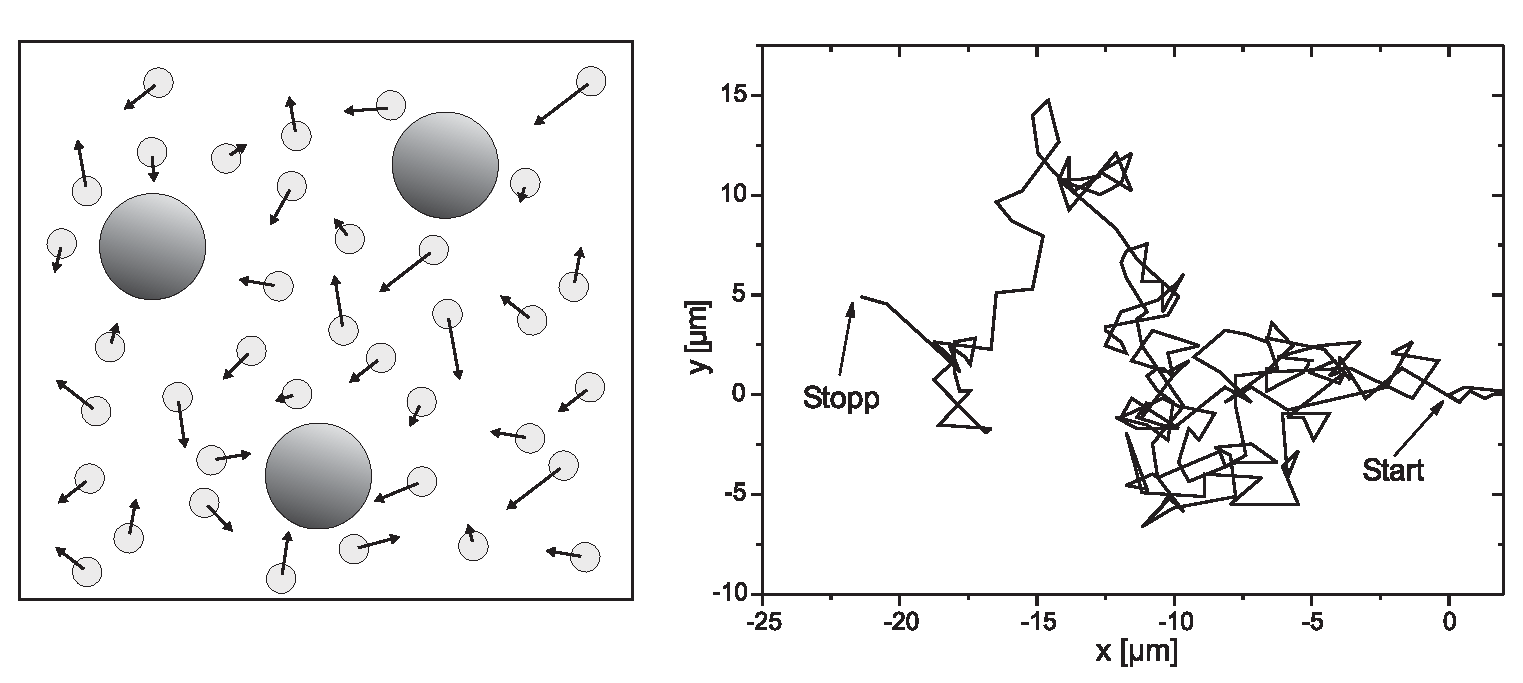
\epsfig{file=249_brown0.eps,width=\textwidth}
\caption{\label{249_brown0}\fontsize{10}{12}\it Links: Modell der
Brownschen Bewegung. Die Molek\"{u}le des umgebenden Mediums sto{\ss}en
aufgrund ihrer thermischen Energie mit den suspendierten
Partikeln, wodurch sich diese auf v\"{o}llig unregelm\"{a}{\ss}igen Bahnen
bewegen. Rechts: Gemessene Bahn eines einzelnen Partikels.}
\end{minipage}
\end{figure}


In diesem Versuch werden Sie die Brownsche Bewegung von
Partikeln suspensiert in Wasser mit einem Mikroskop beobachten
und deren statistische Bewegung untersuchen
(Abbildung~\ref{249_brown0}). Durch Vermessen der Teilchenbahn und
der Berechnung der pro Zeiteinheit auftretenden mittleren
Verschiebung, k\"{o}nnen Sie die Boltzmannkonstante bestimmen.

Eine genaue Bestimmung der Boltzmannkonstante mit Hilfe der
Brownschen Bewegung ist nur bei der Beobachtung sehr vieler
Einzelschritte m\"{o}glich und daher im Praktikum aus Zeitgr\"{u}nden
nicht m\"{o}glich. Bei einer sorgf\"{a}ltigen Durchf\"{u}hrung ist aber eine
Genauigkeit von besser als 10~$\%$ m\"{o}glich. Aus diesem Grund
werden Sie in Teil~II dieses Versuchs ein weiteres Experiment
durchf\"{u}hren, mit dem Sie die Boltzmannkonstante weitaus genauer
bestimmen k\"{o}nnen. Bei diesem Versuch messen Sie das thermische
Rauschen eines ohmschen Widerstands. Dabei ist eine Genauigkeit
von besser als 1~$\%$ m\"{o}glich.

\section{Grundlagen}

\begin{figure}[h]
\begin{minipage}[c]{12cm}
\centering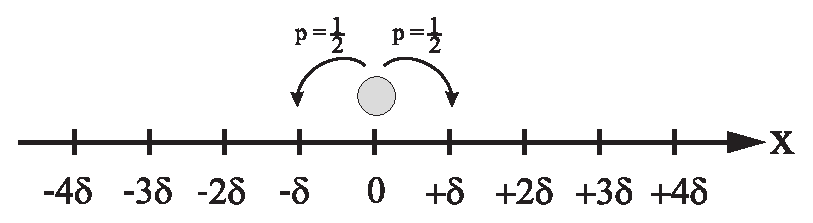
\epsfig{file=249_randomwalk.eps,width=8cm}
\caption{\label{249_randomwalk}\fontsize{10}{12}\it
Eindimensionaler Random-Walk. Bei jedem Sto{\ss} bewegt sich das
Partikel mit der gleichen Wahrscheinlichkeit enweder nach links
oder nach rechts. Die Sprungweite $\delta$ soll bei allen St\"{o}{\ss}en
gleich gro{\ss} sein}
\end{minipage}
\end{figure}




 Die Brownsche Bewegung l\"{a}sst sich mit Hilfe
eines sogenannten Random-Walk Modell quantitativ beschreiben
(Abbildung~\ref{249_randomwalk}). Der Einfachheit halber wollen
wir zun\"{a}chst annehmen, dass sich ein Partikel nur in einer
Dimension, der x-Richtung, bewegen kann. Zum Zeitpunkt $t=0$
befindet sich das Partikel an der Position $x=0$. Wir wollen nun
die Wahrscheinlichkeit berechnen, das Partikel nach der Zeit $t$
im Intervall $[x,x+\Delta x]$ zu finden. Dazu gehen wir von
folgenden Annahmen aus:

\begin{itemize}
    \item Das Partikel erf\"{a}hrt alle $\tau$-Sekunden einen Sto{\ss}.
    Innerhalb der Zeit $t$ treten somit $n=t/\tau$ Sto{\ss}prozesse
    auf.
    \item Bei jedem Sto{\ss} wird das Partikel um die gleiche Distanz
    $\delta$ verschoben. Die Wahrscheinlichkeiten, dass sich das
    Partikel dabei um $+\delta$ nach rechts, bzw. um $-\delta$ nach
    links bewegt, sind gleich gro{\ss}.
    \item Bei mehreren Partikeln h\"{a}ngt die Brownsche Bewegung
    eines einzelnen Partikels nicht von der Bewegung der anderen Partikel
    ab. Jedes Partikel bewegt sich v\"{o}llig unabh\"{a}ngig von den
    anderen, auch dann, wenn sich zwei oder mehrere Partikel sehr
    nahe kommen.
\end{itemize}



Damit sich das Partikel nach $n$-St\"{o}{\ss}en an der Position $x =
m\delta$ befindet, muss es insgesamt $(n+m)/2$-mal in die positive
x-Richtung gelaufen sein und $(n-m)/2$-mal in die negative
Richtung. Dabei ist zu beachten, dass $m$ bei geradem $n$
ebenfalls gerade sein muss und entsprechend  bei ungeradem $n$,
ungerade sein muss.
\\Beispiel: Befindet sich das Partikel nach $n = 10$~St\"{o}{\ss}en an der
Position 6$\delta$ (d.h. $m = 6$), so ist es insgesamt $(n+m)/2$ =
8-mal nach rechts gesprungen und $(n-m)/2$ = 2-mal nach links. Nun
gibt es aber verschiedene M\"{o}glichkeiten, wie das Partikel an die
Position $x = m\delta$ gekommen ist. Es kann z.B. am Anfang
zweimal nach links gesprungen sein und anschlie{\ss}end hintereinander
8~Mal nach rechts gelaufen sein. Insgesamt gibt es

\begin{equation}
   \binom{n}{\frac{1}{2}(n+m)}=\frac{n!}{[\frac{1}{2}(n+m)]!\,[\frac{1}{2}(n-m)]!}
\end{equation}

M\"{o}glichkeiten, welchen Weg das Partikel gelaufen sein k\"{o}nnte. F\"{u}r
unser Beispiel mit $n = 10$ und $m = 6$ ergeben sich
45~verschiedene Schrittfolgen.

Damit k\"{o}nnen wir nun die Wahrscheinlichkeit $P(m;n)$ angeben, mit
welcher sich das Partikel nach $n$-St\"{o}{\ss}en an der Position
$x=m\delta$ befindet. Diese ist gerade durch die
Binomialverteilung\footnote{Siehe auch Versuch~251 \glqq Statistik
des radioaktiven Zerfalls\grqq} gegeben:

\begin{equation}
   P(m;n) = \binom{n}{\frac{1}{2}(n+m)} p^{(n+m)/2}
   (1-p)^{(n-m)/2},
\end{equation}
wobei $p$ die Wahrscheinlichkeit eines einzelnen Sprungs nach
links bzw. nach rechts angibt. Da die Sprungwahrscheinlichkeiten
in beiden Richtungen gleich gro{\ss} sind, gilt $p=1/2$ und somit
\begin{equation}
   P(m;n) = \frac{n!}{[\frac{1}{2}(n+m)]!\,[\frac{1}{2}(n-m)]!}\,\biggl(\frac{1}{2}\biggr)^n.
\end{equation}


In der Regel ist die Zeit $\tau$ zwischen zwei St\"{o}{\ss}en sehr klein,
so dass $n=t/\tau$ bei einer Beobachtungszeit von typischerweise
$t = 1$~s, eine sehr gro{\ss}e Zahl darstellt. F\"{u}r diesen Fall k\"{o}nnen
wir $n!$ und $m!$ mit Hilfe der Stirlingschen Formel

\begin{equation}
    n! = (2\pi n)^{1/2} n^n e^{-n}
\end{equation}
n\"{a}hern. Damit erhalten wir nach einigen Umformungen f\"{u}r die
Wahrscheinlichkeit $P(m;n)$

\begin{equation}\label{249_gauss1}
    P(m;n) = \sqrt{\frac{2}{\pi n}}\, e^{-\frac{m^2}{2n}}.
\end{equation}

Wir wollen nun statt $m$ und $n$, die leicht messbaren Gr\"{o}{\ss}en $x$
und $t$ verwenden. Da $m$ entweder gerade oder ungerade ist, gilt
f\"{u}r $\Delta m$:
\begin{equation}
   \Delta m = \pm 2
\end{equation}
und somit
\begin{equation}
 P(m;n)\frac{\Delta x}{2\delta} = P(x;n) \Delta x
\end{equation}
Substituieren wir $n=t/\tau$ sowie $m=x/\delta$ und definieren
zus\"{a}tzlich die Gr\"{o}{\ss}e $D$:
\begin{equation}\label{249_D}
D=\frac{\delta^2}{2\tau},
\end{equation}
so erhalten wir schlie{\ss}lich f\"{u}r die Wahrscheinlichkeit, ein
Partikel nach der Zeit $t$ innerhalb des Bereichs $[x,x+\Delta x]$
zu finden:
\begin{equation}\label{249_gauss2}
    P(x;t) \Delta x = \frac{\Delta x}{\sqrt{4\pi D t}}\,
    e^{-\frac{x^2}{4 D t}}.
\end{equation}

\begin{figure}[h]
\begin{minipage}[c]{12cm}
\centering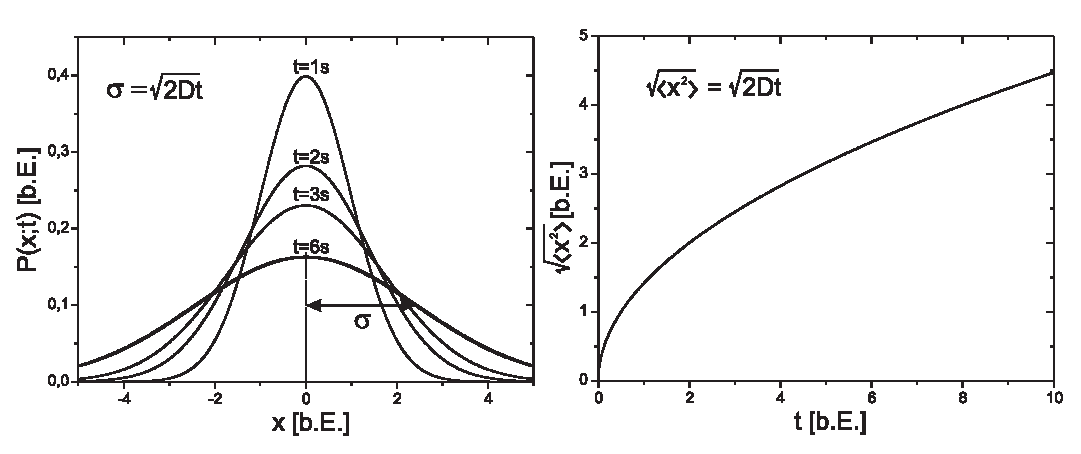
\epsfig{file=249_gauss1.eps,width=\textwidth}
\caption{\label{249_gaussplot}\fontsize{10}{12}\it Links:
Gaussverteilung mit dem Mittelwert $\langle x \rangle = 0$ und der
Varianz $\sigma^2=\langle x^2 \rangle = 2Dt$. Da die Varianz
zeitabh\"{a}ngig ist, wird die Verteilung mit zunehmender Zeit immer
breiter. Rechts: Mittleres Verschiebungsquadrat $\sqrt{\langle x^2
\rangle}$ als Funktion der Zeit.}
\end{minipage}
\end{figure}



P(x;t) in Gleichung~(\ref{249_gauss2}) ist eine Gau{\ss}verteilung
(Abbildung~\ref{249_gaussplot}). Die allgemeine Form solch einer
Verteilung lautet

\begin{equation}\label{249_gauss0}
   G(x;\mu,\sigma)=\frac{1}{\sqrt{2\pi}\,\sigma}\,\text{e}^{-\frac{(\langle x \rangle-x)^2}{2\sigma^2}},
\end{equation}
wobei $\langle x \rangle$ den Mittelwert und $\sigma^2$ die
Varianz, bzw. $\sigma$ die Standardabweichung beschreiben.

Da die Verteilung (\ref{249_gauss2}) symmetrisch zu $x=0$ ist,
verschwindet die mittlere Verr\"{u}ckung $\langle x \rangle$:
\begin{equation}
\langle x \rangle=\int_{-\infty}^\infty x\,P(x;t) dx = 0.
\end{equation}
Dies ist auch sofort einzusehen, da die Wahrscheinlichkeit, dass
das Partikel bei einem Sto{\ss} entweder nach links oder nach rechts
springt, gleich gro{\ss} ist. Der verschwindende Mittelwert $\langle x
\rangle$ ist daher nicht geeignet, die Brownsche Bewegung des
Partikels zu beschreiben. Anders sieht es aus, wenn wir das
mittlere Verschiebungsquadrat $\langle x^2 \rangle$ berechnen:


\begin{equation}
\langle x^2 \rangle=\int_{-\infty}^\infty x^2\,P(x;t) dx = 2Dt =
\sigma^2.
\end{equation}
Das mittlere Verschiebungsquadrat entspricht der Varianz
$\sigma^2=2Dt$ und damit der Breite der Verteilung.

Damit k\"{o}nnen wir das wichtige Ergebnis unserer Untersuchung wie
folgt formulieren:


\setlength{\extrarowheight}{3pt}
\newcolumntype{C}[1]{>{\arraybackslash}p{#1}}
\begin{center}
\begin{tabular}{|C{11cm}|}
  \hline
   Der mittlere Abstand ($\equiv \sqrt{\langle x^2 \rangle}$) eines Partikels vom Ursprungsort, nimmt mit der
Qua\-dratwurzel der Zeit $t$ zu:
\begin{equation}~\label{249_einSmol}
\sqrt{\langle x^2 \rangle} = \sqrt{2Dt} \qquad
\text{Einstein-Smoluchowski-Gleichung}.
\end{equation}
\\\hline
\end{tabular}
\end{center}

Bisher haben wir die Brownsche Bewegung nur in einer Dimension
untersucht. Unser Ergebnis l\"{a}sst sich aber sehr einfach auf
mehrere Dimensionen \"{u}bertragen. Findet die Brownsche Bewegung in
zwei Dimensionen statt, so gilt f\"{u}r das mittlere
Verschiebungsquadrat\footnote{Im mehrdimensionalen Fall schreiben
wir f\"{u}r das mittlere Verschiebungsquadrat ${\langle r^2 \rangle}$
anstatt ${\langle x^2 \rangle}$.} $\langle r^2 \rangle$:

\begin{equation}
\langle r^2 \rangle = \langle x^2 \rangle + \langle y^2 \rangle.
\end{equation}
Da die Brownsche Bewegung isotrop ist, liefert jeder Summand den
Beitrag ${2Dt}$ und somit
\begin{equation}\label{249_2dim}
\sqrt{\langle r^2 \rangle} = \sqrt{4Dt},
\end{equation}
bzw. im Dreidimensionalen:
\begin{equation}
\sqrt{\langle r^2 \rangle} = \sqrt{6Dt}.
\end{equation}

Der Parameter $D$ wird als Diffusionskoeffizient bezeichnet und
ist ein Ma{\ss} f\"{u}r die Beweglichkeit des Partikels im umgebenden
Medium. Nach Einstein ist der Diffusionskoeffizient gegeben durch
\begin{equation}
D = \frac{kT}{f},
\end{equation}

wobei $f$ den Reibungskoeffizienten, $k$ die Boltzmannkonstante
und $T$ die Temperatur der Fl\"{u}ssigkeit darstellen. F\"{u}r
kugelf\"{o}rmige Partikel mit dem Radius $a$, die in einer Fl\"{u}ssigkeit
der Viskosit\"{a}t $\eta$ suspendiert sind, berechnet sich $f$ nach
dem Stokesschen Gesetz (siehe Versuch 212 - Z\"{a}higkeit von
Fl\"{u}ssigkeiten):
\begin{equation}
{f}=6\pi \eta a.
\end{equation}
Damit folgt f\"{u}r den Diffusionskoeffizient nach Stokes-Einstein:
\begin{equation}\label{249_stoke}
D = \frac{kT}{6 \pi \eta a}.
\end{equation}
Diese Beziehung verkn\"{u}pft die makroskopischen Gr\"{o}{\ss}en $\eta$, $a$
und $T$ mit den mikroskopische Gr\"{o}{\ss}en $\delta$ und $\tau$ in
Gleichung~(\ref{249_D}). Einsetzen von (\ref{249_stoke}) in
Gleichung~(\ref{249_2dim}), liefert f\"{u}r das mittlere
Verschiebungsquadrat kugelf\"{o}rmiger Partikel im Zweidimensionalen:

\begin{equation}
\langle r^2 \rangle = \frac{4 k T}{6 \pi \eta a} t.
\end{equation}

Damit haben wir die M\"{o}glichkeit die Boltzmannkonstante
experimentell zu bestimmen. Sind die Gr\"{o}{\ss}en $T, \eta$ und der
Kugelradius $a$ der Partikel bekannt, so kann durch Messung des
mittleren Verschiebungsquadrats die Boltzmannkonstante berechnet
werden: \setlength{\extrarowheight}{3pt}
\newcolumntype{C}[1]{>{\arraybackslash}p{#1}}
\begin{center}
\begin{tabular}{|C{6cm}|}
  \hline
\begin{equation}
k= \frac{6 \pi \eta a }{4  T   t}\langle r^2 \rangle.
\end{equation}
\\\hline
\end{tabular}
\end{center}



\section{Durchf\"{u}hrung}

Lesen Sie \bf bevor\rm~Sie mit den Messungen beginnen, diesen
Abschnitt vollst\"{a}ndig durch! Eine Einf\"{u}hrung in die Bedienung des
Mikroskops und der Messprogramme, erhalten Sie durch den
Versuchsbetreuer.

\begin{figure}[h]
\begin{minipage}[c]{12cm}
\centering\epsfig{file=249_probe.eps,width=8cm}
\caption{\label{249_probe}\fontsize{10}{12}\it Skizze der
Probenfassung. Die ausgestanzte \"{O}ffnung des doppelseitigen
Klebebands wird mit der zu untersuchenden Suspension bef\"{u}llt und
anschlie{\ss}end mit dem Deckglas verschlossen.}
\end{minipage}
\end{figure}
\begin{enumerate}
    \item
\bf Probenpr\"{a}paration:\rm~Sie sollen die Brownsche Bewegung
suspendierter Latex-Partikel in Wasser untersuchen. Um diese mit
dem Mikroskop beobachten zu k\"{o}nnen, ben\"{o}tigen wir eine
Probenfassung, die einerseits dick genug ist, so dass sich die
suspendierten Partikel darin frei bewegen k\"{o}nnen, andererseits
muss diese auch d\"{u}nn genug sein, damit eine Fokussierung mit dem
Mikroskop m\"{o}glich ist. Um dies zu gew\"{a}hrleisten, werden Sie
zun\"{a}chst eine Probenfassung gem\"{a}{\ss} Abbildung~\ref{249_probe}
anfertigen: Auf einen Objekttr\"{a}ger wird ein doppelseitiges
Klebeband aufgebracht, in dessen Mitte zuvor ein Loch ausgestanzt
wurde. In diese \"{O}ffnung wird die Probenfl\"{u}ssigkeit eingef\"{u}llt und
mit einem Deckglas verschlossen.  Das doppelseitige Klebeband
erf\"{u}llt dabei zwei Aufgaben: Zum einen vergr\"{o}{\ss}ert dieses das
Probenvolumen, so dass sich die suspendierten Partikel frei
bewegen k\"{o}nnen, zum anderen dient es zur Abdichtung der
Fl\"{u}ssigkeit, wodurch ungewollte Str\"{o}mungen durch
Verdunstungsprozesse unterdr\"{u}ckt werden.

\begin{figure}
\begin{minipage}[c]{12cm}
\centering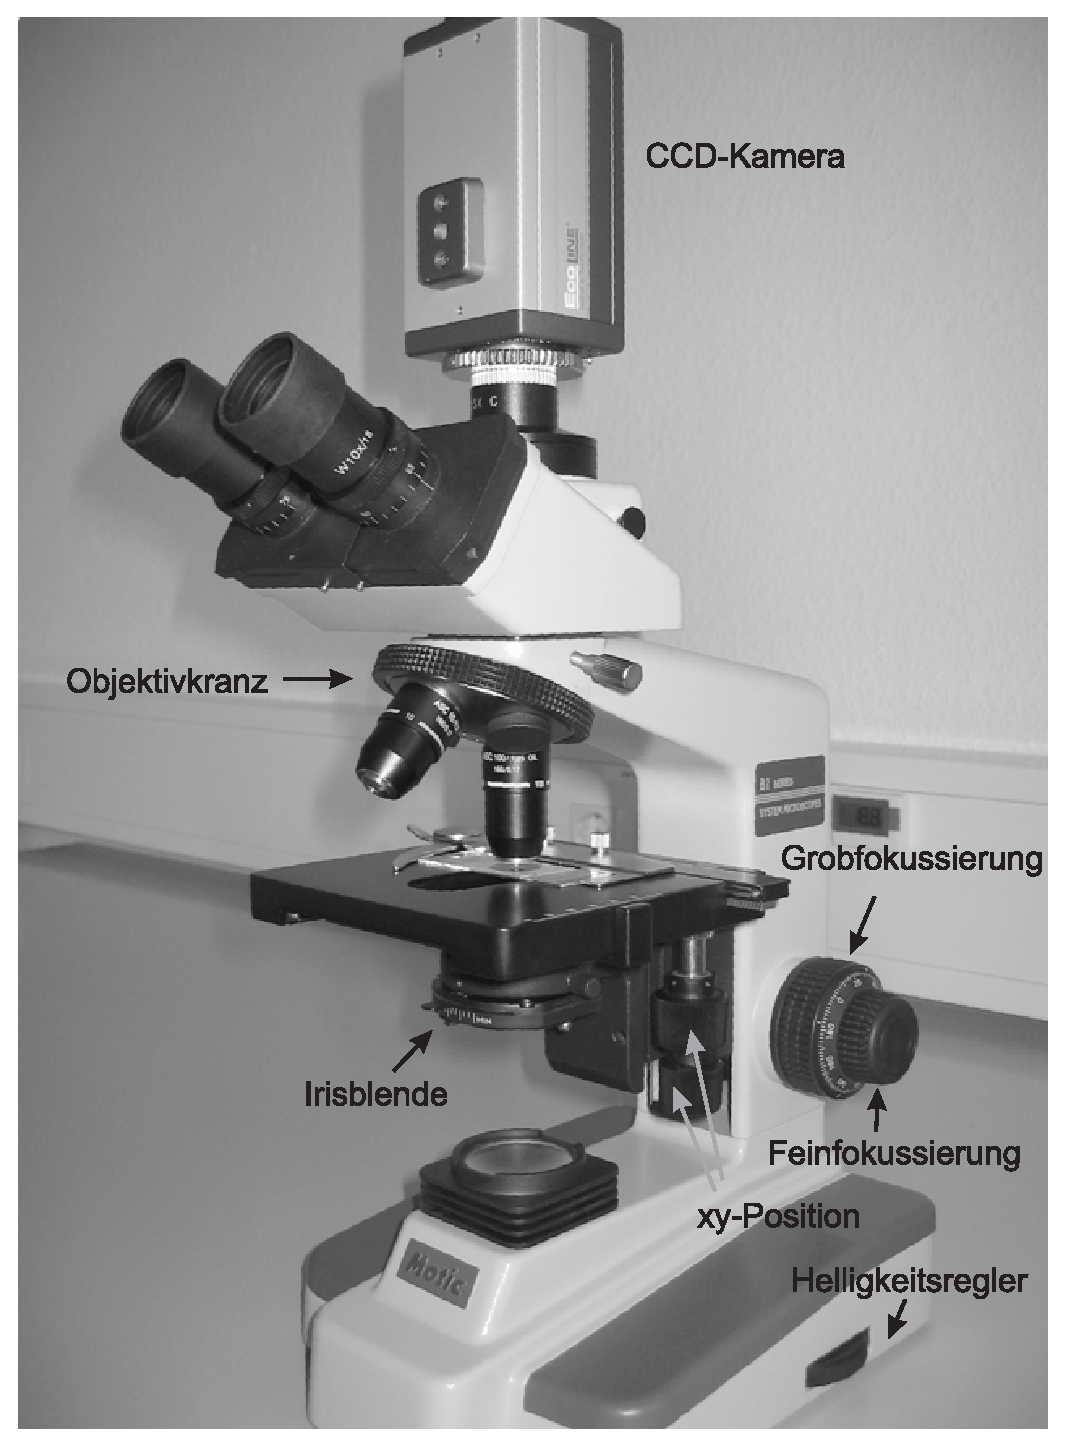
\epsfig{file=249_Mikroskop.eps,width=9cm}
\caption{\label{249_Mikroskop}\fontsize{10}{12}\it
Bedienungselemente des Mikroskops.}
\end{minipage}
\end{figure}


Fertigen Sie vor Versuchsbeginn stets eine neue Probe an!
Schneiden Sie dazu ein St\"{u}ck doppelseitiges Klebeband passend auf
die Gr\"{o}{\ss}e des Deckglases (24~mm~$\times$~32~mm) zurecht und
stanzen Sie mit dem Locheisen zentrisch ein Loch in das Klebeband
(Holzunterlage verwenden!). Anschlie{\ss}end kleben Sie das Klebeband
mittig auf den Objekttr\"{a}ger und entfernen die Abdeckfolie.
Sch\"{u}tteln Sie die Flasche mit der Probenfl\"{u}ssigkeit gut durch und
pipettieren Sie 250~$�l$ der Probenfl\"{u}ssigkeit in die ausgestanzte
\"{O}ffnung des Klebebands. Werfen Sie die Pipettenspitze nach
Gebrauch sofort in den Abfall. Der Durchmesser der Partikel ist
auf der Flasche angegeben. Notieren Sie diesen Wert in Ihr
Protokollheft. Legen Sie nun das Deckglas auf das doppelseitige
Klebeband und dr\"{u}cken Sie es mit einem Papiertuch vorsichtig an.
Dabei darf ruhig etwas von der Fl\"{u}ssigkeit herausflie{\ss}en.
Allerdings d\"{u}rfen sich keine (gr\"{o}{\ss}eren) Luftblasen in der
Fl\"{u}ssigkeit bilden! Trocknen Sie die Probe mit einem Papiertuch ab
und und geben Sie auf die Mitte des Deckglases \bf einen
Tropfen\rm~Immersions\"{o}l. Spannen Sie nun die Probe auf den
Mikroskoptisch (Abbildung~\ref{249_Mikroskop}) ein.  Am
Objektivkranz des Mikroskops w\"{a}hlen Sie das Objektiv 100/1.25~oil
(100-fache Vergr\"{o}{\ss}erung, Numerische Apertur NA=1,25)
aus.\\
\\\it Frage: Wozu wird das Immersions\"{o}l ben\"{o}tigt?\rm\\
\\
Schalten Sie die Mikroskopbeleuchtung ein. Bewegen Sie nun den
Mikroskoptisch \bf VORSICHTIG\rm~mit Hilfe der Fokuseinstellung
(\it Grobfokussierung\rm~in Abbildung~\ref{249_Mikroskop}) soweit
in Richtung des Objektivs, bis dieses \bf gerade\rm~den \"{O}ltropfen
ber\"{u}hrt. Versuchen Sie nun durch \bf
vorsichtiges\rm~Scharf\-stellen mit Hilfe des Feinreglers,
einzelne Partikel der Suspension zu beobachten. Die $xy$-Position
der Probe k\"{o}nnen sie mit Hilfe der beiden $xy$-Einstellr\"{a}der
verstellen. Die Fokussierung ist bei der gew\"{a}hlten 1000-fachen
Vergr\"{o}{\ss}erung nicht ganz einfach. Sollten Sie hierbei Probleme
haben, wenden Sie sich an den Versuchsbetreuer.

\bf Achtung:\rm~Bei der Versuchsdurchf\"{u}hrung k\"{o}nnen systematische
Fehler auftreten, die unbedingt zu vermeiden sind:
\begin{itemize}
\item \"{U}berzeugen Sie sich, dass  Sie wirklich nur ein einziges
Partikel beobachten. Manchmal kann es vorkommen, dass zwei oder
mehrere Partikel \glqq zusammenkleben\grqq. Dies l\"{a}sst sich gut
erkennen, indem man etwas den Fokus variiert.

\item Auf keinen Fall d\"{u}rfen Sie w\"{a}hrend der Messung die
$xy$-Position des Objekttisches verstellen. Auch Ersch\"{u}tterungen
des Mikroskops m\"{u}ssen unbedingt vermieden werden.
    \item  Beim Nachfokussieren d\"{u}rfen Sie mit dem Objektiv auf
    keinen Fall das Deckglas ihrer Probe ber\"{u}hren. Der dadurch
    erzeugten Druck, w\"{u}rde die Partikel verdr\"{a}ngen und
    somit die eigentliche Brownsche Bewegung verf\"{a}lschen. Sollten
    Sie beim Nachfokussieren eine abrupte Partikelbewegung
    beobachten, so m\"{u}ssen Sie sich ein anderes, \glqq h\"{o}her
    gelegenes\grqq~Partikel suchen, dessen Position Sie ohne
    Ber\"{u}hrung des Deckglases scharf stellen k\"{o}nnen.

     \item Die Probe muss sich im thermischen Gleichgewicht
     befinden. Ist dies nicht der Fall, so treten
     Konvektionsstr\"{o}me auf, die wiederum die Brownsche Bewegung
     verf\"{a}lschen. Zudem ist es m\"{o}glich, dass die Probe schlecht
     pr\"{a}pariert wurde: Ist die Suspension nicht vollst\"{a}ndig mit
     dem Klebeband abgedichtet, so k\"{o}nnen durch Verdunstungsprozesse
     ebenfalls ungew\"{u}nschte Str\"{o}mungen in der Probe auftreten. Warten Sie
     daher zur Temperierung der Probe einige Minuten ab, bevor Sie
     mit der Messung beginnen. Sollte dann immer noch eine Str\"{o}mungsbewegung
     erkennbar sein, so m\"{u}ssen Sie gegebenenfalls eine neue Probe vorbereiten.
     Wenden Sie sich in diesem Fall an Ihren Betreuer.
\end{itemize}


\item \bf Aufnahme einer Bildfolge: \rm~Starten Sie vom Desktop
aus das Programm \it Kamera.exe\rm. Dieses Programm nimmt in einem
festen Zeitabstand ein Bild auf und speichert dieses auf dem
Computer. Tragen Sie im Messprogramm f\"{u}r den Zeitabstand 1~s ein.
Schalten Sie die Option \it Bilder speichern\rm~zun\"{a}chst ab.

Suchen Sie sich nun ein Partikel aus, in dessen unmittelbarer
Umgebung sich keine anderen Partikel befinden und stellen Sie die
$xy$-Position des Mikroskoptisches so ein, dass sich das
ausgew\"{a}hlte Partikel im Zentrum des Mikroskopbildes befindet. Zur
Verbesserung des Kontrastes sollten Sie die Irisblende am
Kondensor auf die Position \it MIN\rm~stellen.

Da die Brownsche Bewegung nicht nur in der $xy$-Bildebene, sondern
auch in $z$-Richtung erfolgt, wird es passieren, dass das zu
beobachtende Partikel aus dem Fokus l\"{a}uft und somit nicht mehr
sichtbar wird. Um dem entgegenzuwirken, m\"{u}ssen Sie  die
Fokussierung des Mikroskops mit dem Feinregler dauernd
nachjustieren. Dies erfordert einiges an Feingef\"{u}hl und besonders
Konzentration.

F\"{u}hren Sie zun\"{a}chst eine Probemessung durch: Damit sich die Probe
durch die Mikroskopbeleuchtung nicht zus\"{a}tzlich aufheizt, drehen
Sie die Helligkeit auf das Minimum zur\"{u}ck. Die Kamera ist auch bei
dieser Minimalbeleuchtung empfindlich genug, kontrastreiche Bilder
zu liefern. Starten Sie das Programm durch Anklicken des Pfeils in
der linken oberen Ecke und versuchen Sie der Bewegung eines
Partikels \"{u}ber mehrere Minuten auf dem Monitor zu folgen. Sobald
das Partikel auch nur leicht unscharf zu erkennen ist, m\"{u}ssen Sie
sofort mit dem Feintrieb des Mikroskops den Fokus vorsichtig
nachstellen. \bf Das Partikel muss
w\"{a}hrend der ganzen Zeit eindeutig erkennbar sein!\rm\\

Wenn Sie nun genug \"{U}bung im Nachfokussieren erlangt haben und die
zuvor genannten Punkte bez\"{u}glich der systematischen Fehler
ber\"{u}cksichtigt haben, k\"{o}nnen Sie mit der eigentlichen Messung
beginnen. Stoppen Sie das Messprogramm. Schalten Sie die Option
\it Bilder speichern\rm~ein und starten Sie erneut das Programm.
\bf Insgesamt ist jede Sekunde und mindestens 150~mal, ein Bild
aufzunehmen.\rm~Entfernen Sie nach der Messung die Probe und
werfen Sie diese in den Abfall. \bf Achtung: Auf keinen Fall
d\"{u}rfen Sie nach Beendigung der Messung das Programm nochmals
starten. Ihre zuvor aufgenommenen Bilder w\"{u}rden sonst
\"{u}berschrieben werden.\rm

\item \bf Notieren Sie die Zimmertemperatur.\rm~Das Thermometer
ist auf der R\"{u}ckseite des Mikroskops angebracht.

\item \bf Eichung des Abbildungsma{\ss}stabs:\rm~Um sp\"{a}ter die
Position des Partikels ausmessen zu k\"{o}nnen, m\"{u}ssen Sie den
Abbildungsma{\ss}stab des Mikros\-kops bestimmen. Benutzen Sie dazu
das ausliegende Objektmikrometer. Geben Sie einen Tropfen
Immersions\"{o}l auf das Objektmikrometer und legen Sie dieses auf den
Mikroskoptisch. Stellen Sie vorsichtig den Fokus ein und
positionieren Sie den Mikroskoptisch so, dass Sie den Ma{\ss}stab
gem\"{a}{\ss} Abbildung~\ref{249_Eichung} erkennen k\"{o}nnen. Beenden Sie das
Messprogramm und starten Sie das Programm \it Eichung.exe\rm.
Optimieren Sie nochmals die Bildsch\"{a}rfe und speichern Sie dann das
Eichbild. Reinigen Sie das Objektmikrometer mit einem Papiertuch
und legen Sie es zur\"{u}ck in die Aufbewahrungsbox.

\begin{figure}
\begin{minipage}[c]{12cm}
\centering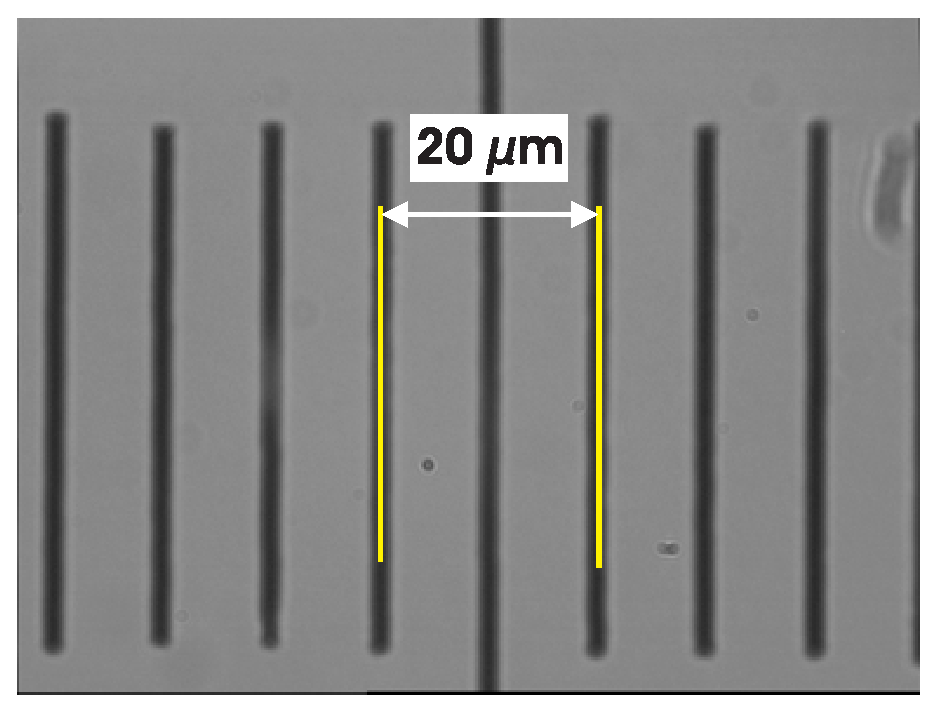
\epsfig{file=249_Eichung.eps,width=9cm}
\caption{\label{249_Eichung}\fontsize{10}{12}\it Eichung des
Abbildungsma{\ss}stabs mit einem Objektmikrometer. Die Distanz
zwischen zwei Teilstrichen betr\"{a}gt 10~$\mu$m. }
\end{minipage}
\end{figure}

\item \bf Vermessung der Partikelpositionen:\rm~Starten Sie das
Programm \it Auswertung.exe\rm~vom Desktop aus. Um die
Partikelpositionen zu bestimmen, m\"{u}ssen Sie wissen, wie viele
Bildpixel einem Mikrometer entsprechen. Laden Sie dazu das zuvor
gespeicherte Eichbild (Schalter \it Eichbild laden\rm~im Feld \it
Eichung\rm) und messen Sie mit Hilfe des Cursors den Pixelabstand
\"{u}ber eine Distanz von 20~$\mu$m (Abbildung~\ref{249_Eichung}). Die
Pixelwerte werden im Feld \it Marker\rm~angezeigt. Den Cursor
k\"{o}nnen Sie zum einen mit der Maus bewegen, als auch mit den
Steuerpfeilen unter dem Bildfeld (Abbildung~\ref{249_Programm}).
Tragen Sie den gemessenen Pixelabstand in das Feld \it
Eichung\rm~ein.

\begin{figure}[h]
\begin{minipage}[c]{12cm}
\centering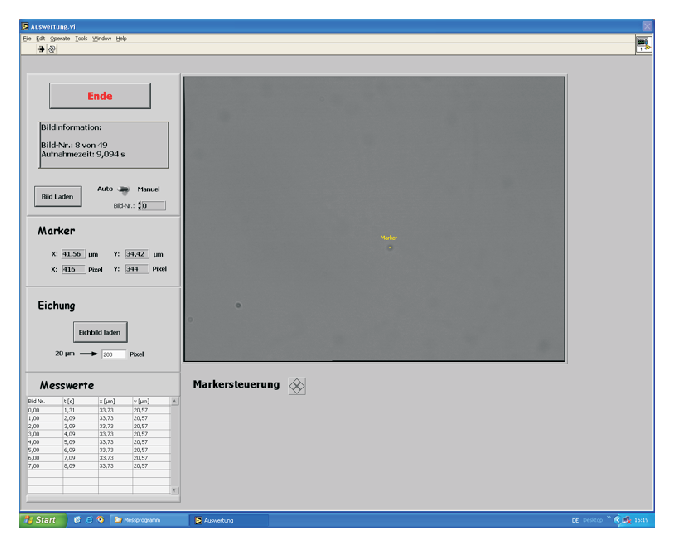
\epsfig{file=249_Programm.eps,width=\textwidth}
\caption{\label{249_Programm}\fontsize{10}{12}\it Bedienoberfl\"{a}che
des Programms zur Ausmessung der Partikelpositionen der
aufgenommenen Bilder.}
\end{minipage}
\end{figure}

Nach dieser Eichung k\"{o}nnen Sie mit der Vermessung der
Partikelpositionen Ihrer aufgenommenen Bilder beginnen. Laden Sie
das erste Bild, indem Sie auf den Schalter \it Bild
laden\rm~klicken (der daneben liegende Schalter soll auf der
Position \it Auto\rm~stehen). Verfahren Sie den Marker nun so,
dass dieser sich \bf exakt\rm~in der Mitte des Partikels befindet.
Die entsprechenden Koordinaten werden im Feld \glqq
Marker\grqq~angezeigt. Wenn Sie nun erneut auf den Schalter \it
Bild laden\rm~klicken, wird die zuvor ausgemessene
Partikelposition gespeichert, im Feld \it Messwerte\rm~angezeigt,
und das n\"{a}chst folgende Bild geladen. Vermessen Sie so die
Partikelposition aller aufgenommenen Bilder. Das Programm wird
automatisch gestoppt, wenn Sie die Partikelposition des letzten
aufgenommenen Bildes bestimmt haben. Die Messwerte werden unter
\verb"C:\Messungen\Messung.dat" als Textdatei gespeichert.

\item Fangen Sie sofort mit der Auswertung der Messdaten an.
\end{enumerate}




\section{Auswertung}

Die Auswertung erfolgt mit der auf dem Messrechner installierten Software Origin.
Achtung: Da es im Laborbuch nicht m\"{o}glich ist nachzuvollziehen, welche Rechnungen Sie mit Origin durchgef\"{u}hrt haben, muss bei allen Spaltenberechnungen die entsprechende Rechenvorschrift (Formel) im Laborbuch kommentiert werden!

\begin{enumerate}
\item Berechnung des mittleren Verschiebungsquadrates und dessen Fehler.\\
\\Die Messdaten sind in der Datei \verb"Messung.dat" im Ordner Messungen auf dem Desktop gespeichert. F\"{u}r jede Messung enth\"{a}lt die Datei drei Eintr\"{a}ge: Die Zeit in Sekunden sowie die x und die y-Koordinaten in $\mu$m.  Starten Sie Origin und importieren Sie die Datei \verb"Messung.dat":  \verb"Datei" $\rightarrow$ \verb"Import" $\rightarrow$ \verb"Einzelnes ASCII".
Beschriften Sie die Spaltenk\"{o}pfe angemessen und speichern Sie das Projekt unter einem sinnvollen Namen.

\begin{figure}[h]
\begin{minipage}[c]{12cm}
\centering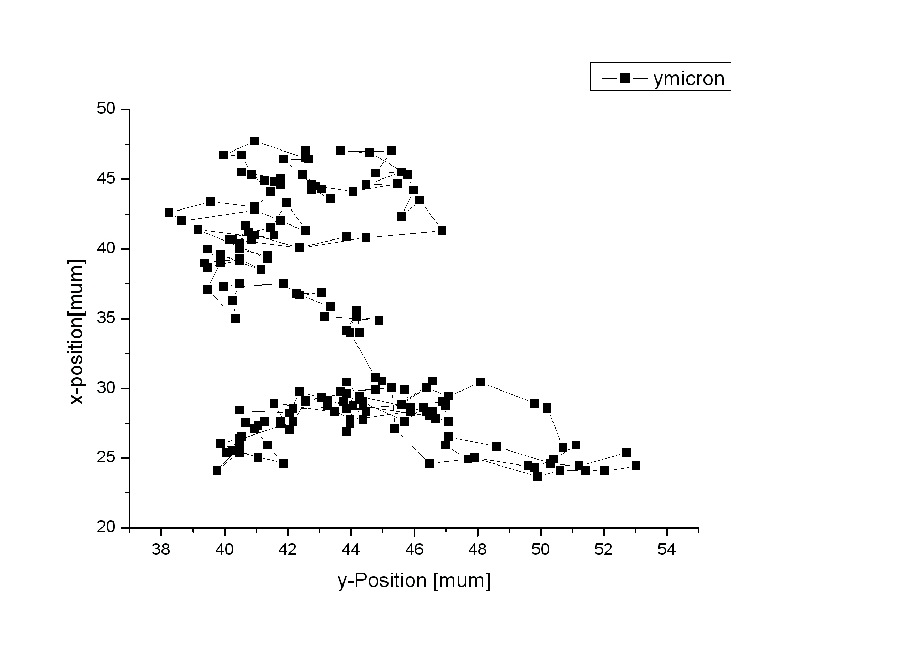
\epsfig{file=223_auswertung1.eps,width=\textwidth}
\centering\caption{\label{223_auswertung1}\fontsize{10}{12}\it
Bewegung eines Partikels.}
\end{minipage}
\end{figure}

Verschaffen Sie sich einen grafischen Eindruck von der Wanderung des Partikels. Setzen Sie dazu die Spalte mit den $x$-Koordinaten als X und die f\"{u}r die $y$-Koordinaten als Y und zeichnen Sie diese Daten als Punkt-Liniendiagramm. Drucken Sie das Diagramm aus und f\"{u}gen Sie es in Ihr Protokollheft ein.
Das Diagramm sollte so \"{a}hnlich aussehen wie in Abbildung~\ref{223_auswertung1}.

Die Messdaten geben die absoluten Koordinaten an, wir brauchen aber die
Koordinaten\"{a}nderungen $\Delta x_i = x_{i+1} - x_i$   und $\Delta y_i = y_{i+1} - y_i$ sowie deren Quadrate. Erweitern
Sie die Tabelle daher um sechs Spalten: Zeitdifferenz $\Delta t, \Delta x, \Delta y, \Delta x^2,
\Delta y^2$ und $r^2=\Delta x^2+\Delta y^2$. Die Differenzen k\"{o}nnen Sie wie folgt berechnen:
Die zu berechnende Spalte markieren, Rechtsklick auf den Spaltenkopf $\rightarrow$ \verb"Spaltenwerte errechnen" ausw\"{a}hlen. Geben Sie anschlie{\ss}end folgende Formel ein: col(t)[i+1]- col(t)[i]. F\"{u}r \glqq t\grqq~in \glqq col(t)\grqq~m\"{u}ssen Sie nat\"{u}rlich Ihren gew\"{a}hlten Spaltennammen eintragen Wiederholen Sie diese Berechnungen f\"{u}r die anderen Spalten. In der letzten Spalte kann nat\"{u}rlich keine Differenz mehr berechnet werden, in ihr erscheint ein Strich.

Als n\"{a}chstes brauchen wir Mittelwerte und Fehler der Messwerte in den neu berechneten
Spalten. In Origin lassen sich diese Werte mit Hilfe der Spaltenstatistik berechnen:
Die zu berechnende Spalte markieren, Rechtsklick auf den Spaltenkopf $\rightarrow$ \verb"Spaltenstatistik" $\rightarrow$ \verb"Dialog oeffnen" ausw\"{a}hlen.
Klicken Sie im sich \"{o}ffnenden Fenster auf  \verb"Zu berechnende Mengen" und danach auf \verb"Momente" und w\"{a}hlen Sie die ben\"{o}tigte Gr\"{o}{\ss}en aus.
Das Ergebnisfenster liefert f\"{u}r alle ausgew\"{a}hlten Spalten die gew\"{u}nschten Resultate.
Notieren Sie sich in einer Tabelle f\"{u}r jede Messgr\"{o}{\ss}e die folgenden Werte:
Mittelwert, Standardabweichung, SE des Mittelwerts, die minimalen und maximalen Werte.

Damit ist die mittlere quadratische Abweichung $\langle r^2 \rangle$ und dessen Fehler $\Delta\langle r^2 \rangle$ bestimmt.
Berechnen Sie hieraus die Boltzmannkonstante und die Diffusionskonstante $D$ mit den jeweiligen Fehlern.

\item Kontrollverteilung\\
\\Nach Gleichung~\ref{249_gauss2} ist die Wahrscheinlichkeit,
ein Partikel nach der Zeit $t$ innerhalb des Bereichs $[x,x+\Delta
x]$ zu finden durch eine Gau{\ss}verteilung gegeben. \"{U}berpr\"{u}fen Sie
dies, indem Sie die gemessenen Partikelverschiebungen in ein
Histogramm eintragen. Da die Brownsche Bewegung isotrop ist,
k\"{o}nnen Sie sowohl die Verschiebungen $\Delta x$ als auch die
Verschiebungen $\Delta y$ gemeinsam in das gleiche Histogramm
eintragen. Kopieren Sie gemeinsam die Daten $\Delta x$ und $\Delta y$ in eine neue Spalte. Markieren Sie mit der linken Maustaste den Spaltenkopf. W\"{a}hlen Sie durch Rechtsklick auf den Spaltenkopf die Option \verb"Zeichnen" $\rightarrow$ \verb"Statistikdiagramme" $\rightarrow$ \verb"Histogramm" aus. \"{O}ffnen Sie das Datenblatt des Histogramms: Rechtsklick ins Histogramm $\rightarrow$ \verb" Gehe zu Klassierungsdaten". Zeichnen Sie mit diesen Daten ein S\"{a}ulendiagramm der Verteilung.


Berechnen Sie mit Hilfe der Spaltenstatistik den Mittelwert $\mu$ sowie die
Standardabweichung $\sigma$ der Verteilung und zeichnen Sie anhand
dieser beiden Werte eine Gau{\ss}kurve in das S\"{a}ulendiagramm mit ein. Am einfachsten geht dies, wenn Sie die nichtlineare Fitfunktion in Origin verwenden und alle
Fitparameter festhalten.
Stimmt der berechnete Mittelwert mit dem theoretischen Wert
\"{u}berein? Berechnen Sie aus der Breite $\sigma$ der Verteilung die
Diffusions\-konstante und die Boltzmannkonstante und vergleichen
Sie diese mit dem zuvor bestimmten Werten. Drucken Sie das
S\"{a}ulendiagramm mit der berechneten Gau{\ss}kurve aus.
\item Kumulative Verteilung der Verschiebungsquadrate.\\
\\Nach Gleichung~(\ref{249_einSmol}) ist das mittlere
    Verschiebungsquadrat $\langle r^2 \rangle$ proportional zur
    Zeit.

    Berechnen Sie eine neue Spalte im Arbeitsblatt mit der kumulativen Verteilung von $\langle r^2 \rangle$.
 Nutzen Sie hierzu folgenden Trick:
  \begin{itemize}
    \item 	Tragen Sie in die erste Zeile der neuen Spalte die Summe der Zeilen 1 und 2 von  $\langle r^2 \rangle$ von Hand ein.
    \item  Die anderen Zeilen berechnen Sie gem\"{a}{\ss} den Vorgaben in Abbildung~\ref{223_auswertung2} (Rechtsklick auf den Spaltenkopf $\rightarrow$ \verb"Spaltenwerte errechnen" ausw\"{a}hlen).
  \end{itemize}


 \begin{figure}
\begin{minipage}[c]{12cm}
\centering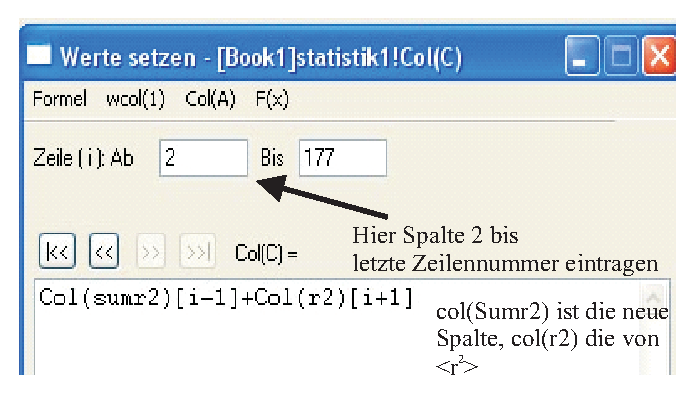
\epsfig{file=223_auswertung2.eps,width=8cm}
\centering\caption{\label{223_auswertung2}\fontsize{10}{12}\it
Berechnung der kumulativen Verschiebung.}
\end{minipage}
\end{figure}

Stellen Sie diese Werte in einem neuen Diagramm als Funktion der Zeit dar. Es sollte sich ein linearer Zusammenhang gem\"{a}{\ss} Abbildung~\ref{223_auswertung3} ergeben. Fitten Sie eine Gerade an die Daten. Aus der Steigung kann wieder die Diffusionskonstante bestimmt werden. Stimmt sie mit den anderen Messungen \"{u}berein?

 \begin{figure}
\begin{minipage}[c]{12cm}
\centering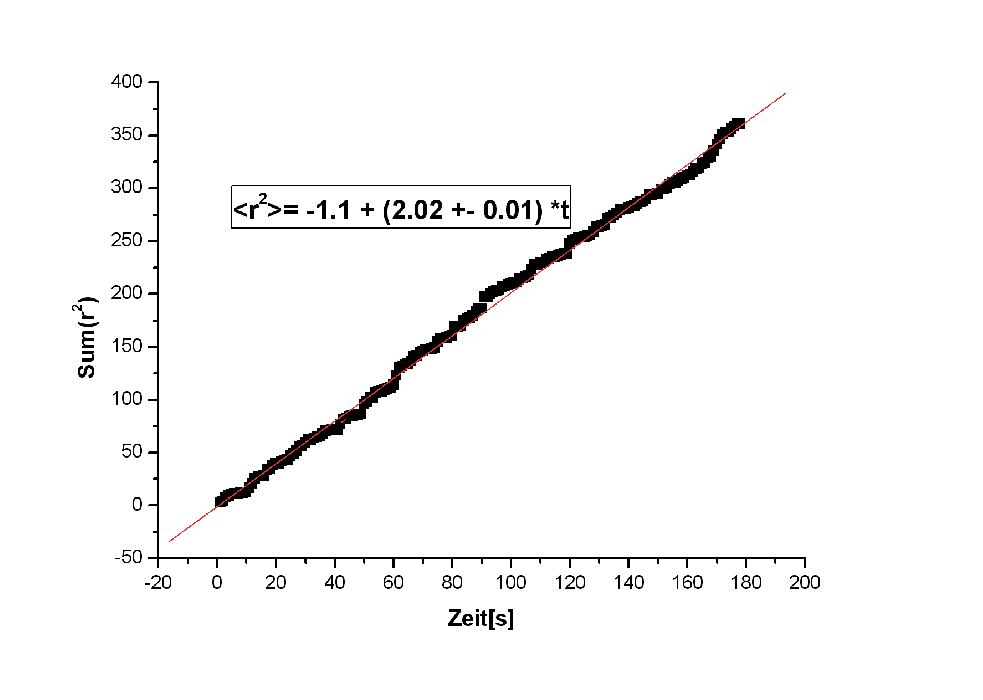
\epsfig{file=223_auswertung3.eps,width=\textwidth}
\centering\caption{\label{223_auswertung3}\fontsize{10}{12}\it
Kumulative Verschiebung eines Partikels.}
\end{minipage}
\end{figure}

\end{enumerate}




\begin{figure}
\begin{minipage}[c]{22cm}
\centering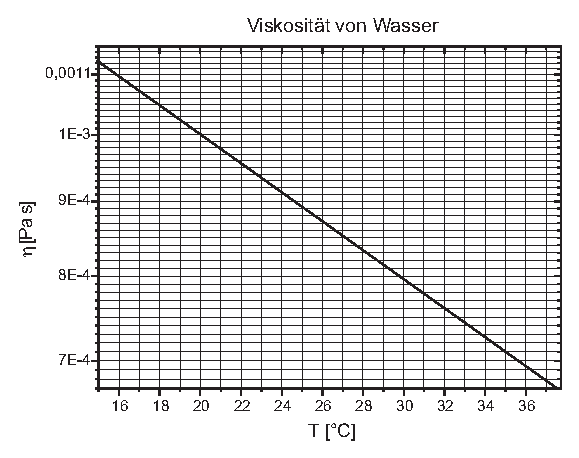
\epsfig{file=249_Viskositaet.eps,width=18cm}
\centering\caption{\label{249_Viskositaet}\fontsize{10}{12}\it
Temperaturabh\"{a}ngigkeit der Viskosit\"{a}t von Wasser.}
\end{minipage}
\end{figure}



\end{document}
\newpage
\section*{}

\newpage
\section*{} 